\documentclass[a4paper,11pt]{paper}
\author{Quelli della B1}
\usepackage[utf8]{inputenc}
\usepackage[italian]{babel}
\usepackage{graphicx}
\usepackage[colorlinks=true,linkcolor=blue]{hyperref}
\graphicspath{{./images/}}

\def\code#1{\texttt{#1}}

\title{Networking}

\begin{document}

\maketitle
\newpage
\tableofcontents
\newpage

\subsection{Introduzione}
Gioara
\subsubsection{I protocolli}
\subsubsection{Il modello ISO OSI}
\subsubsection{Internet protocol suite (TCP/IP)}

\newpage

\section{Livello Fisico}
Nonostante l'amministratore di rete non abbia la possibilità di influirvi direttamente, è importante descrivere lo strato fisico poiché esso influenza significativamente le prestazioni della rete.
\subsection{Terminologia}
\subsubsection{Informazione} 
L'informazione è una grandezza misurabile in bit. In particolare, \[Q=log_{2}m\] dove $Q$ è il numero di bit necessari per rappresentare l'informazione relativa ad $m$ possibili stati. 

\subsubsection{Codice}
Al fine di rappresentare l'informazione in maniera tale da renderne più semplice la gestione, un codice associa sequenze di bit a caratteri. I codici che godono della più ampia diffusione sono:
\begin{itemize}
\item ASCII (American Standard Code for Information Interchange, 7 bit estesi a 1 byte)
\item BCD (Binary-Coded Decimal)
\item AIKEN 
\item Gray
\item EBCDIC (Extended Binary Coded Decimal Code, 8 bit), in uso presso le banche
\end{itemize}
\subsubsection{Segnale}
Si dice \textit{segnale} una grandezza fisica variabile nel tempo corrispondente un'informazione. Un segnale \textbf{analogico} varia in modo continuo nel tempo ed ha infiniti livelli di intensità; un segnale \textbf{digitale} varia invece in modo discreto e ha solo due livelli di intensità. Ogni tipo di dato può essere rappresentato in entrambe le maniere e può essere convertito da analogico a digitale e viceversa.
\\\\Fra i segnali analogici assumono particolare rilevanza i \textbf{segnali sinusoidali}, ossia segnali che variano nel tempo secondo una legge del tipo \[u=Usen(\omega t+\Phi )\] dove $u$ è l'ampiezza istantanea, $U$ l'ampiezza massima, $\omega $ la frequenza e $\Phi $ lo sfasamento. L'intervallo di tempo impiegato dall'onda per tornare allo stesso livello d'intensità è detto \textit{periodo}.\\\\ 
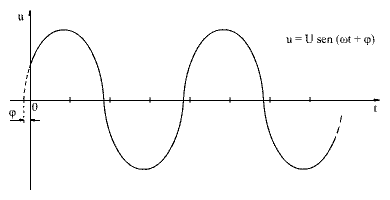
\includegraphics[scale=0.5]{segnali_sin.png}
\subsubsection{Lunghezza d'onda}
\subsubsection{Spettro}
\subsubsection{Banda}
\subsection{Filtri}

\subsection{Flusso di trasmissione}
\subsubsection{Simplex}
\subsubsection{Half-Duplex}
\subsubsection{Full-Duplex}

\subsection{Modulazione}
\subsubsection{Ad onda continua}
\subsubsection{Impulsiva}
\subsubsection{Digitale}

\subsection{Qualità delle trasmissioni} non so se mi piace qui
\subsubsection{Ritardo}
\subsubsection{Tempo di risposta}
\subsubsection{Throughput}
\subsubsection{Latenza}
\subsubsection{Jitter}

\subsection{Alterazioni del segnale}
\subsubsection{Attenuazione}
\subsubsection{Distorzione}
\subsubsection{Rumore}
\subsubsection{Interferenza}

\subsection{Limiti alla velocità di trasferimento}
\subsubsection{Classificazione dei canali trasmissivi}
\subsubsection{Teorema di Nyquist}
\subsubsection{Teorema di Shannon}
\subsubsection{Velocità di modulazione}

\newpage
\section{Livello di Collegamento}

\subsection{Tipi di trasmissione}
\subsubsection{Sincrona}
\subsubsection{Asincrona}
\subsubsection{Orientata al carattere} forse non è collegamento
\subsubsection{Orientata al bit}

\subsection{Controlo degli errori}
\subsubsection{Ridondanza}

\subsection{Protocolli primario-secondario}
\subsubsection{RTS-CTS}
\subsubsection{XON-XOF}
\subsubsection{ARQ}

\subsection{Protocolli internet}
\subsubsection{ARP}
\subsubsection{RARP}
\subsubsection{NDP}
\subsubsection{MAC}

\subsection{Ethernet}


\newpage
\section{Livello di Rete}

\subsection{Terminologia}
\subsubsection{Rete}
\subsubsection{DTE}
\subsubsection{DCE}
\subsubsection{CPE}
\subsection{Tipologie di rete}
\subsection{Topologia delle reti}
\subsection{Qualità della rete}
\subsection{Routing}
\subsubsection{Tabella di routing}
\code{netstat -nr}

\subsection{Internet Protocol (IP)}


\subsection{Protocolli di routing dinamico}
\subsubsection{ICMP}
\subsubsection{IGMP}
\subsubsection{RIP}
\subsubsection{OSPF}


Claudio
\newpage
\section{Livello di Trasporto}
\subsection{Protocolli}
\subsubsection{TCP}
\subsubsection{UDP}
\newpage

\section{Livello Applicazione}
\subsection{Servizi di Rete}
Tommaso
\subsubsection{Telnet}
\subsubsection{FTP}
\subsubsection{SSH}
\subsubsection{BGP}
\subsubsection{DHCP}
\subsubsection{DNS}
\subsubsection{HTTP}

\end{document}
